\documentclass[14pt,a4paper]{extreport}
\usepackage[utf8]{vietnam}
\usepackage{graphicx}
\usepackage{xcolor}
\usepackage{wrapfig}
\usepackage{multicol}
\usepackage{fancyhdr}
\usepackage{fancybox}
\usepackage{iflang}
\usepackage{caption}
\usepackage{amsmath}
\DeclareMathOperator*{\argmax}{argmax}
\DeclareMathOperator*{\argmin}{argmin}
\usepackage[left=2.5cm, right=2.50cm, top=2.50cm, bottom=2.50cm]{geometry}
\pagestyle{fancy}
\fancyhf{}
\fancyhead[LE,RO]{\thepage}
\fancyhead[LO]{\small{\itshape{}}}
\graphicspath{ {./images/} }
\begin{document}


	\thispagestyle{empty}
\thisfancypage{
	\setlength{\fboxsep}{10pt}
	\fbox}{}
\begin{center}
	\begin{large}
		TRƯỜNG ĐAI HỌC BÁCH KHOA HÀ NỘI
	\end{large} \\
	\begin{large}
		VIỆN CÔNG NGHỆ THÔNG TIN VÀ TRUYỀN THÔNG
	\end{large} \\
	
	\textbf{--------------------  *  ---------------------}\\[1.5cm]
	
\includegraphics[scale=0.25]{12}
	\\
	\vspace{1.5cm}
	{\fontsize{17pt}{1}\selectfont  Môn học}\\[0.3cm]
	{\fontsize{20pt}{1}\selectfont 	Phân tích và thiết kế thuật toán}\\[0.9cm]
	{\fontsize{17pt}{1}\selectfont  Tên đề tài}\\[0.5cm]
	{\fontsize{23pt}{1}\selectfont \textbf{Maximum Induced Matching}}\\[1.3cm]
\end{center}
\vspace{0.7cm}
%\hspace{2.7cm}
\begin{center}
	{\fontsize{17pt}{1}
	\selectfont Giảng viên hướng dẫn: } \hspace{1pt}
\textbf{\parbox[t]{6cm}{
		\selectfont TS. Đỗ Phan Thuận\\
	}
}
\end{center}

\hspace{1.59cm}
{\fontsize{17pt}{1}
	\selectfont Sinh viên thực hiện: } \hspace{1pt}
\textbf{\parbox[t]{6cm}{
		\selectfont Lâm\ Xuân\ Thư\\		
	}
}

\hspace{5.0cm}
{\fontsize{12pt}{1}
		\selectfont MSSV : } \hspace{1pt}
	\textbf{\parbox[t]{6cm}{
			\selectfont  20153709\\
		}
	}

\hspace{5.4cm}
{\fontsize{17pt}{1}
	\selectfont Lớp: } \hspace{1pt}
\textbf{\parbox[t]{6cm}{
		\selectfont KSTN\ CNTT\ K60\\
	}
}\\[20pt]

\vspace{0.7cm}
\begin{center}
	
	{\fontsize{17pt}{1}\selectfont Hà Nội, \today}
	%{\fontsize{12pt}{1}\selectfont November, 29$^{th}$, 2017}
\end{center}




\newpage
\thispagestyle{empty}

\begin{abstract}
	
Trong đồ thị G, một tập induced matching là một tập các cạnh trong G mà khoảng cách giữa hai cạnh bất kì ít nhất phải bằng hai (tính theo số cạnh). Bài toán Maximum Induced Matching là bài toán đi tìm tập induced matching có số lượng phần tử lớn nhất. Bài toán này là NP-khó đối với các đồ thị tổng quát. Trên một số lớp đồ thị đặc biệt, bài toán Maximum Induced Matching có thể giải được trong thời gian đa thức hoặc thời gian tuyến tính.

Trong bài này em xin trình bày về giới thiệu bài toán Maximum Induced Matching và các thuật toán giải Maximum Induced Matching trên các lớp đồ thị hình thang, đồ thị interval, đồ thị Chordal, Interval, Circular arc, Cây, đồ thị Asteroidal triple-free, đồ thị Hamiltonian và các đồ thị có Matching và Induced Matching cùng kích cỡ lớn nhất. 

\end{abstract}

\tableofcontents 
%\listoffigures
\newpage
\setlength{\parindent}{4em}
\setlength{\parskip}{1em}
\renewcommand{\baselinestretch}{1.5}



\chapter{Giới thiệu}
\section{Induced Matching và bài toán Maximum Induced Matching}

Xét G = (V, E) là đồ thị với tập các đỉnh V và tập các cạnh E. Tập các cạnh $ M \subset E $ được gọi là một matching nếu không tồn tại 2 cạnh bất kì trong M có đỉnh chung. Kích thước lớn nhất của một matching trong đồ thị G kí hiệu là$  m(G) $ và có thể tính được trong thời gian đa thức. Induced matching  là matching mà không tồn tại 2 cạnh nào trong nó được nối bởi một cạnh trong E. Kích thước lớn nhất của một Induced matching được kí hiệu là $ im(G) $. Hiển nhiên ta thấy $ im(G) \leq m(G) $. 

Bài toán Maximum induced matching (MIM) là bài toán đi tìm $ im(G) $ với đồ thị G cho trước.  Bài toán này được giới thiệu bởi tác giả Cameron và đã được nghiên cứu phát triển trong nhiều năm qua. Maximum induced matching là bài toán NP-hard trên đồ thị tổng quát, kể cả trên đồ thị hai phía. Mặt khác, Maximum induced matching có thể giải trong thời gian đa thức đối với một số lớp đồ thị đặc biệt, như chordal graphs, trapezoid graphs và k-interval-dimension graphs, polygon-circle graphs (bao gồm chordal graphs, circular-arc graphs, circle graphs và outerplanar graphs), AT-free graphs và weakly chordal graphs.

\begin{figure}
	\centering
	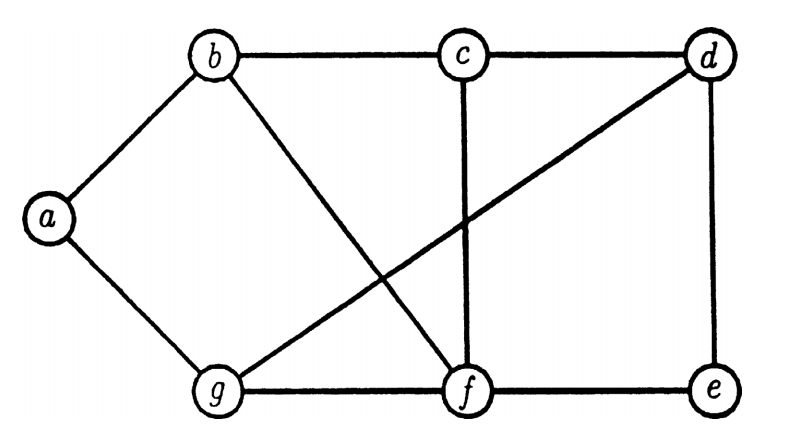
\includegraphics[scale=.39]{mim}
	\caption{Một đồ thị với một MIM là {(a, b), (d, e)} có cỡ là 2}
\end{figure}

\section{Line graph và Square graph}

\textit{Line graph} và \textit{Square graph} là các lớp đồ thị đặc biệt mà các tính chất của chúng của thể được áp dụng trong bài toán Maximum Induced Matching để việc tính toán trở lên thuận lợi hơn. Định nghĩa Line graph và Square graph được trình bày sau đây.

\textit{Line graph}:  Line graph của đồ thị G kí hiệu là \textit{L(G)}, là đồ thị có mỗi đỉnh là một cạnh trong G, hai đỉnh trong L(G) được nối với nhau bởi một cạnh nếu hai cạnh tương ứng trong G kề nhau. 

\textit{Square of G}: kí hiệu là $ G^{2} $, là đồ thị có tập đỉnh là tập đỉnh của G, hai đỉnh trong $ G^{2} $ được nối với nhau bởi một cạnh nếu nếu hai đỉnh tương ứng trong G có khoảng cách (tính theo số cạnh) không lớn hơn 2.

Kí hiệu $ [L(G)]^{2} $ là G*.

Nhận xét: từ định nghĩa trên dễ dạng nhận thấy: mỗi \textit{induced matching} trong G tương ứng với một \textit{independent set} trong G*.

\begin{figure}
	\centering
	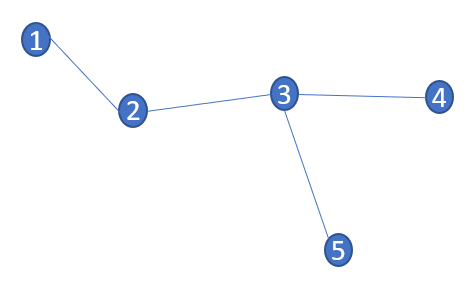
\includegraphics[scale=.6]{g}
	\caption{Một đồ thị G1 bất kì}
\end{figure}

\begin{figure}
	\centering
	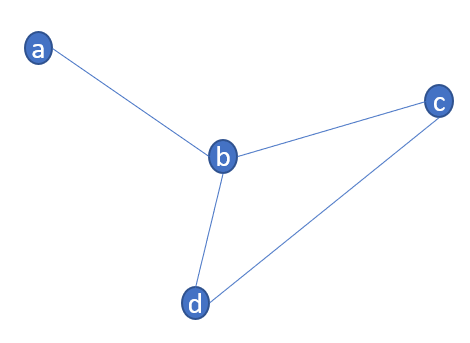
\includegraphics[scale=.5]{lineg}
	\caption{Line graph của G1}
\end{figure}

\begin{figure}
	\centering
	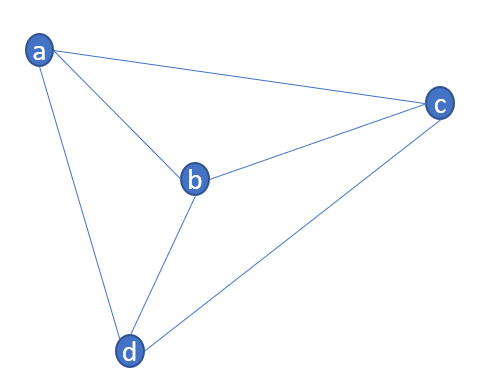
\includegraphics[scale=.5]{squarelineg}
	\caption{Square của Line của G1}
\end{figure}

\chapter{Thuật toán thời gian đa thức đối với một vài lớp đồ thị quen thuộc}
\section{Một vài lớp đồ thị quen thuộc}

\begin{itemize}
	\item \textit{Chordal graph}: đồ thị G là chordal graph  nếu với mọi chu trình có nhiều hơn hoặc bằng 4 đỉnh trong G thì có ít nhất một chord. 
	\item \textit{Interval graph}: xét một đường thẳng cho trước và các đoạn thẳng nằm trên đường thẳng đó. Một đồ thị G là interval graph có mỗi đỉnh của nó tương ứng với một đoạn thẳng trên đường thẳng, hai đỉnh có cạnh nối nếu hai đoạn thẳng tương ứng với hai đỉnh có giao nhau khác rỗng. 
	\item \textit{Circular arc graph}: xét các cung tròn trên một đường tròn. Một đồ thị là Circular arc graph có mỗi đỉnh tương ứng với một cung tròn, hai đỉnh có cạnh nối nếu hai cạnh tương ứng giao nhao khác rỗng.
\end{itemize}

\begin{figure}
	\centering
	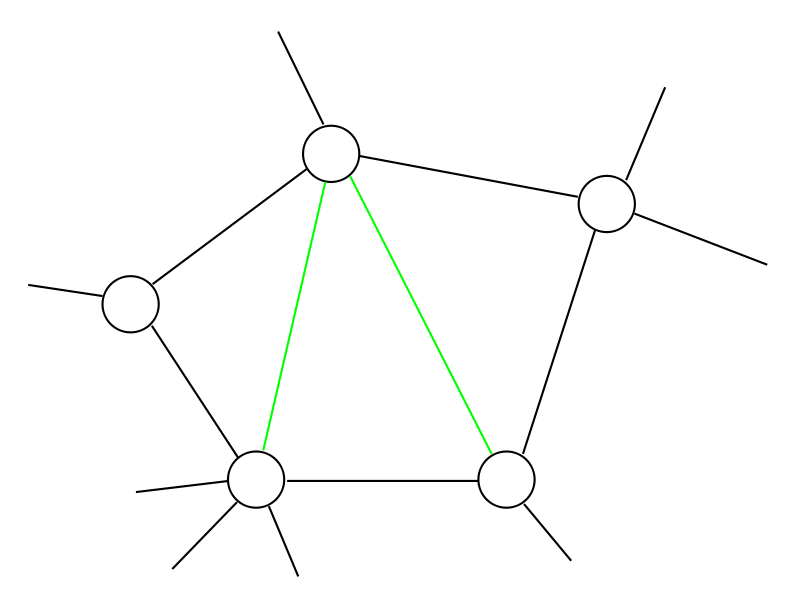
\includegraphics[scale=.39]{chordal}
	\caption{Một đồ thị chordal}
\end{figure}

\begin{figure}
	\centering
	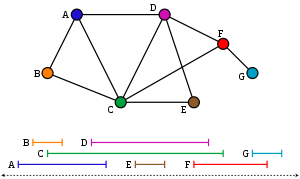
\includegraphics[scale=1]{interval}
	\caption{Một đồ thị interval}
\end{figure}

\begin{figure}
	\centering
	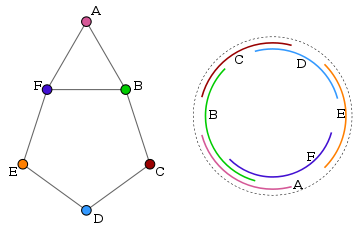
\includegraphics[scale=.9]{circular}
	\caption{Một đồ thị circula arc}
\end{figure}

\section{Thuật toán tìm Induced Matching lớn nhất}

\textbf{Định lí 2. 2}: 
\begin{enumerate}
	\item Nếu G là một Chordal graph, thì G* là một Chordal graph.
	\item Nếu G là một Interval graph, thì G* là một Interval graph.
	\item Nếu G là một Circular arc graph, thì G* là một Circular arc graph.
\end{enumerate}
	
Trong khi đó bài toán tìm maximum independent set đã được chỉ ra là có thể giải được trong thời gian đa thức đối với các đồ thị interval [13, 14], circular arc [11, 15, 1] và chordal [7]. \\
Nhắc lại rằng: mỗi \textit{induced matching} trong G tương ứng với một \textit{independent set} trong G*.\\
 Kết hợp với định lí 2.2 ta có thể dẫn tới kết luận: tồn tại các thuật toán thời gian đa thức cho bài toán MIM đối với Chordal graph, Interval graph, Circular arc graph.

Phương pháp tìm MIM này có thể áp dụng tương tự trên đồ thị hình thang. Ta sẽ đi vào tìm hiểu cụ thể trong phần tiếp theo.


\chapter{Đồ thị hình thang}
\section{Định nghĩa}

Xét hai đường thẳng song song. Một hình thang giữa hai đường thẳng này được xác định bởi hai điểm nằm trên đường thẳng dưới và hai điểm nằm trên đường thẳng trên.\\
 Một đồ thị là \textit{đồ thị hình thang} nếu tồn tại một tập các hình thang tương ứng với tập các đỉnh của đồ thị, sao cho hai đỉnh được nối bởi một cạnh nếu hai hình thang tương ứng giao nhau. 

\begin{figure}
	\centering
	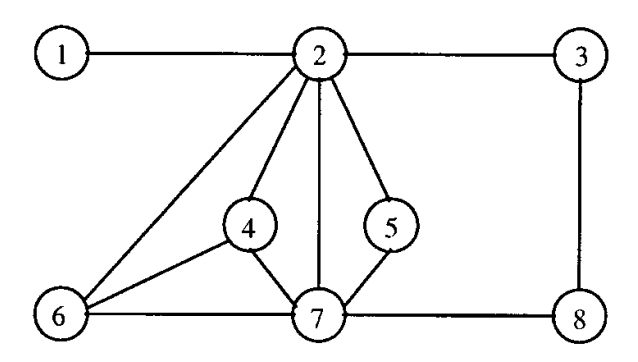
\includegraphics[scale=.5]{trapezoid}
	\caption{Một đồ thị hình thang G2}
\end{figure}

\begin{figure}
	\centering
	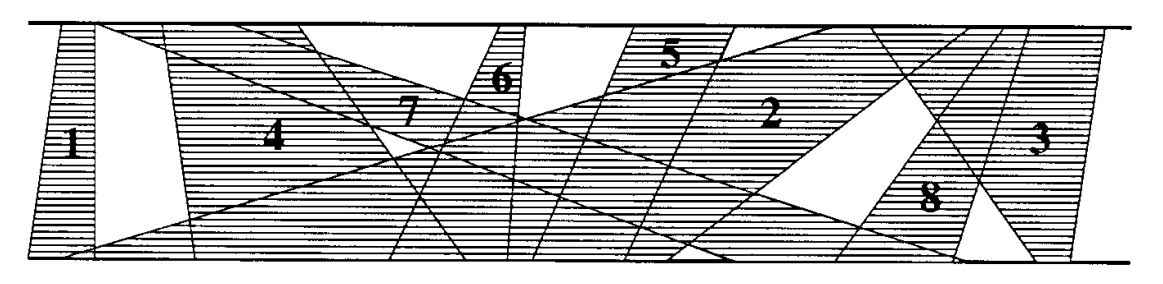
\includegraphics[scale=.5]{trapezoid2}
	\caption{Biểu diễn các hình thang giao nhau của G2}
\end{figure}

\section{Maximum induced matching trên đồ thị hình thang}

\textbf{Định lí}: Nếu G là một đồ thị hình thang, thì G* là một đồ thị hình thang [21].\\
\textbf{Hệ quả}: Tìm kiếm một tập maximum induced matching trên một đồ thị hình thang có thể thực hiện trong thời gian đa thức.\\
\textbf{Chứng minh}: Felsner [5] đã đưa ra thuật toán thời gian tính O(n log n) cho bài toán tìm maximum independent set trong đồ thị hình thang, áp dụng thuật toán này vào G* sẽ dẫn đến kết quả cần chứng minh.

\chapter{Cây}
Cây là đồ thị liên thông không có chu trình.\\
Không giống như các lớp đồ thị vừa nêu ở mục trước, cây G không có tính chất vẫn là cây khi chuyển sang G*. 

\begin{figure}
	\centering
	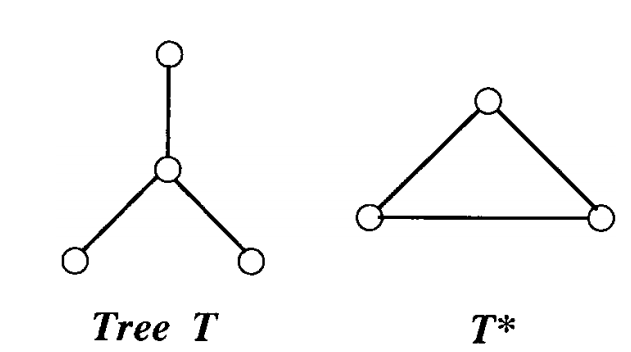
\includegraphics[scale=.5]{tree}
	\caption{T* không còn là cây}
\end{figure}

Tuy nhiên, do cây là một trường hợp đặc biết của đồ thị chordal, nên với mọi cây T, thì T* là một chordal graph. Do đó, tồn tại thuật toán thời gian đa thức để tìm MIM trên cây. Lưu ý rằng thuật toán này không chạy với thời gian tuyến tính. Trong phần này sẽ trình bày một thuật toán khác có thể tìm ra số lượng phần tử của Maximum induced matching trên cây trong thời gian \textit{tuyến tính}.

Số lượng phần tử (size) của Maximum induced matching trên cây có thể tính trong thời gian tuyến tính theo thuật toán như sau:\\
Giả sử T là cây đã cho. Chọn một đỉnh bất kì trong T là gốc. \\
Kí hiệu:\\
$ T_{v} $ là cây con gốc tại v.\\
$ \mu_{s}(T_{v}) $ là size của MIM tại $ T_{v} $.\\
$ \mu_{s1}(T_{v}) $ là size của MIM tại $ T_{v} $ sao cho không có cạnh nào trong matching chạm v.\\
$ \mu_{s2}(T_{v}) $ là size của MIM tại $ T_{v} $ sao cho không có cạnh nào trong matching chạm một con của v.\\
Công thức đệ quy:\\

$ \mu_{s1}(T_{v}) = \sum_{u }\mu_{s}(T_{u}) $ \\

$ \mu_{s2}(T_{v}) = \sum_{u }\mu_{s1}(T_{u}) $ \\

$ \mu_{s}(T_{v}) = \max (\mu_{s1}(T_{v}), \max_{u} (1 +  \mu_{s2}(T_{u}) + \sum_{w } \mu_{s1}(T_{w})))$ \\


\chapter{Đồ thị Asteroidal triple-free}

Ở đây ta chỉ xét các đồ thị vô hướng, không có khuyên và cạnh lặp.

\section{Asteroidal triple-free}
Cho đồ thị G = (V, E), láng giềng mở N(u) của một đỉnh u thuộc V là tập hợp $ {v \in V \arrowvert {u, v} \in E } $,và láng giềng đóng N[u] là $ {u} \cup N(u) $. Láng giềng của một cạnh e = (x, y) là tập các cạnh với ít nhất một đỉnh nằm trong   $ N(x) \cup N(y) $.\\
\textit{Asteroidal triple} (AT) là tập 3 đỉnh mà 2 đỉnh bất kì được nối bởi một đường tránh láng giềng gần của đỉnh còn lại. AT-free là đồ thị không chứa AT.\\
\textit{Asteroidal set}: tập $ A \subseteq V $ là asteroidal set nếu với mọi đỉnh $  a \in A $, tập A \ {a} được chứa trong một thành phần liên thông của G – N[a]. Mọi asteroidal set là một independent set. Asteroidal number là số lượng lớn nhất các phần tử của một asteroidal set. Kí hiệu A(s): họ đồ thị có asteroidal number nhiều nhất là s. AT-free graph thuộc A(2).

\section{Line-Asteroidal triple-free graphs}
Line-asteroidal set là một tập các cạnh $ F \subseteq E $, sao cho với mọi $ e \in F$ sao cho $ F \ {e} $ được chứa trong một thành phần liên thông của G – N(e). Mọi line-asteroidal set là một tập induced matching.\\
Line-asteroidal triple (AT) là tập 3 cạnh mà 2 cạnh bất kì được nối bởi một đường tránh láng giềng gần của cạnh còn lại. LAT-free là đồ thị không chứa LAT.\\
Asteroidal-index là số lượng lớn nhất các phần tử của một line-asteroidal set.\\
Kí hiệu L(s) là họ đồ thị có asteroidal index không vượt quá s. Như vậy, LAT-free graph thuộc L(2).\\

\textbf{Định lí 5.2.a}: nếu F là một line-asteroidal set trong G, thì các cạnh tương ứng với F trong G* tạo thành một tập asteroidal.\\

\textbf{Định lí 5.2.b}: nếu A là một asteroidal set trong G*, thì tập các cạnh tương ứng với A trong G là một line-asteroidal set.\\

\textbf{Định lí 5.2.c}: $ G \in (s) $ (s >1) khi và chỉ khi $ G* \in A(s)$. Đặc biệt khi s = 2 ta có, G là LAT-free khi và chỉ khi G* là AT-free.\\

Broersma chứng minh rằng tìm maximum independent set trong một đồ thị n đỉnh và asteroidal number không lớn hơn s có thể thực hiện trong thời gian $ O(n^{s+2}) $. Áp dụng thuật toán này vào đồ thị G* với G là đồ thị có asteroidal index bị chặn ta dẫn tới hệ quả: Bài toán MIM trên đồ thị có asteroidal index giới hạn có thể giải trong thời gian đa thức. 

\chapter{Đồ thị có Matching và Induced Matching cùng kích cỡ lớn nhất}

\section{Thuật toán IM}
Theo định nghĩa về tập Matching  và Induced matching có thể thấy mỗi tập  Induced matching là một tập Matching, do đó hiển nhiên rằng số phần tử của tập Induced matching lớn nhất luôn nhỏ hơn hoặc bằng số phần tử của tập Matching lớn nhất, tức là $ im(G) \leq m(G) $. Trong khi đó m(G) đã được chính minh có thể tính được trong thời gian đa thức. Vì vậy với những đồ thị có im(G) = m(G) thì MIM có thể giải được trong thời gian đa thức.

Phần này sẽ trình bày về thuật toán IM kiểm tra xem một đồ thị G cho trước liệu im(G) có bằng m(G) hay không. Nếu câu trả lời là có thì đồng thời thuật toán sẽ trả về số lượng phần tử của tập Induced matching lớn nhất.

Thuật toán có sử dụng các định nghĩa sau. Một đỉnh v gọi là một lá nếu bậc của nó bằng 1 (có đúng một đỉnh kề). Một cạnh e được gọi là một cạnh lá nếu ít nhất một đỉnh của nó là lá. Một cạnh e được gọi là một cạnh tam giác nếu hai đỉnh của nó có bậc là hai và có chúng một đỉnh láng giềng.

\textbf{Nội dung thuật toán IM}:\\
\begin{itemize}
	\item Input: đồ thị G
	\item Output: im(G) hoặc kết luận im(G) < m(G) .
\end{itemize}

\begin{enumerate}
	\item Nếu G không liên thông, áp dụng IM cho từng thành phần liên thông của G;\\
	nếu G chỉ có 1 đỉnh, đặt$  I = \phi $ và tới bước 7;\\
	nếu G là một clique và có nhiều hơn 1 đỉnh, đặt I là một cạnh bất kì của G và tới bước 7.
	\item đặt$  I = \phi $
	\item Với mọi đỉnh có nhiều hơn một cạnh lá kề với nó: giữ lại một cạnh lá duy nhất và xoá các cạnh lá còn lại.
	\item Với mọi cạnh e, nếu e là cạnh lá hoặc cạnh tam giác thì thêm e vào I.
	\item Nếu I rỗng, đặt I là cạnh bất kì của G.
	\item 	Nếu I không phải Induced Matching, thông báo im(G) < m(G) và kết thúc.
	\item 	Xác định m(G).
	\item 	Nếu | I | < m(G) , thông báo im(G) < m(G) và kết thúc; nếu không trả về | I | và kết thúc.
\end{enumerate}

\textit{\textbf{Đánh giá thời gian tính của thuật toán IM:}}\\
Gọi số cạnh của G là m, số đỉnh của G là n. Bước 3 và bước 4 có thể thực hiện trong thời gian O(m). Xét bước 6, nếu số lượng phần tử của tập I lớn hơn n/2 có thể kết luận ngay I không phải Induced Matching. Do đó, bước 6 có thể thực hiện trong thời gian $ O(n^{2}) $. Ở bước 7 ta sử dụng thuật toán của của Micali and Vazirani có thời gian là$  O(n^{1/2}m) $. Vậy, thời gian tính của toàn bộ thuật toán IM là $ O(max\{n^{2}, n^{1/2}m\}) $.

\section{Đặc trưng của các đồ thị có IM bằng M}
Xét các định nghĩa sau:
\begin{itemize}
	\item \textit{Sao}: là một đồ thị hai phía đầy đủ gồm n+1 đỉnh, các cạnh nối một đỉnh với tất cả các đỉnh còn lại.
	\item \textit{Tam giác}: là một đồ thị đầy đủ gồm 3 đỉnh.  
	\item \textit{Lá}: một đỉnh trong đồ thị có bậc bằng 1.
	\item \textit{Cạnh lá}: cạnh có đỉnh là lá.
	\item \textit{Pendant triangle}: là một \textit{tam giác} có 2 đỉnh có bậc 2 và cạnh còn lại có bậc lớn hơn 2.
\end{itemize}
Kathie Cameron, Tracy Walker đã rút ra các đặc trưng chung của các đồ thị có tập Induced Matching lớn nhất và tập Matching lớn nhất có cùng số lượng phần tử qua định lí sau:

\textbf{Định lí}: Cho G là một đồ thị liên thông. \textit{im(G) = m(G)} khi và chỉ khi G là một \textit{sao} hoặc một \textit{tam giác} hoặc bao gồm một đồ thị hai phía đầy đủ \textit{B} với ít nhất một cạnh và các lớp màu đen và trắng, với ít nhất một cạnh lá gắn với mỗi đỉnh màu đen của \textit{B}, và có thể có một số \textit{Pendant triangle} gắn với cạnh trắng của B.

\chapter{Đồ thị Hamiltonian}

Xét đồ thị G = (V, E). \textit{Đường đi Hamiltonian} là một đường đi P trong G mà mỗi đỉnh trong V xuất hiện đúng một lần trong P.\textit{ Chu trình Hamiltonian} là một chu trình C trong G mà mỗi đỉnh trong V xuất hiện đúng một lần trong C. \textit{Đồ thị Hamiltonian} là đồ thị chứa chu trình Hamiltonian.

\textbf{Định lí 7}: cho G là đồ thị chứa hamiltonian path, H = Line(G). Khi đó, im(H) = [n / 3], với n là số đỉnh của G.

\textbf{\textit{Chứng minh}}:
Một IM trong H tương ứng với một tập các path trên 3 đỉnh phân biệt trong G. Do đó: $ im(H) \leq [n / 3] $ .\\
Nhóm các nhóm gồm 3 đỉnh liên tiếp trên Hamiltonian path của G, mỗi nhóm tương ứng với một cạnh trong một IM trong H. 
Do đó: $ im(H) \geq [n / 3] $ .\\
 Suy ra: im(H) = [n / 3] .

\textbf{Hệ quả}: MIM có thể giải được trong thời gian đa thức đối với line graph của đồ thị có chứa Hamiltonian path.

\textit{\textbf{Chứng minh}}: Xét H là một đồ thị có n đỉnh và m cạnh là đồ thị line của một đồ thị G có chứa đường đi Hamiltonian nào đó. Một đồ thị G’ sao cho      line(G’) = H có thể xác định trong thời gian O(n + m) [25]. Đồ thị G’ có thể không chứa đường đi Hamiltonian nhưng G và G’ có cùng số đỉnh n’. Theo định lí 7 có im(H) = [n’ / 3]. Vậy số lượng phần tử của tập induced matching lớn nhất trong H có thể tính trong thời gian tuyến tính.

\chapter{Tổng kết}
Bài toán Maximum induced matching (MIM) là bài toán đi tìm tập induced matching lớn nhất với đồ thị G cho trước.  Bài toán này được giới thiệu bởi tác giả Cameron và đã được nghiên cứu phát triển trong nhiều năm qua. Maximum induced matching là bài toán NP-hard trên đồ thị tổng quát.

Tuy nhiên, Maximum induced matching có thể giải trong thời gian đa thức đối với một số lớp đồ thị đặc biệt. Với các đồ thị G thuộc lớp đồ thị Chordal, Interval, Circular arc, Trapezoid (đồ thị hình thang), đồ thị có asteroidal index giới hạn (trường hơp đặc biết là LAT-free) có thể tìm MIM bằng cách chuyển về bài toán tìm tập Indepedent lớn nhất trên đồ thì Square của Line của G khi mà ta đã có các thuật toán thời gian đa thức để giải.\\
Đối với đồ thị là \textit{cây}, có thể tìm MIM trong thời gian đa thức vì cây là trường hợp đặc biệt của đồ thị \textit{chordal}; nhưng có thuật toán tốt hơn với thời gian tuyến tính.\\
Đối với những đồ thị có Maximum Matching bằng Maximum Induced Matching có thể giải bằng cách đi tìm Maximum Matching (tồn tại thuật toán thời gian đa thức tìm Maximum Matching trên đồ thị tổng quát).\\
Đồ thị Hamiltonian khác với các đồ thị trên khi bài toán MIM trên đồ thị Hamiltonian vẫn là bài toán NP-hard nhưng trên đồ thị Line của nó lại có thể giải được trong thời gian đa thức.
 





\begin{thebibliography}{9} 

	\bibitem{latexcompanion}  J. Edmonds, Paths, trees, and flowers, Canad. J. Math. 1 (1965), 449-467.
	\bibitem{latexcompanion}  K. Cameron, Induced matchings, Discrete Appl. Math. 24 (1989), 97-102.
	\bibitem{latexcompanion}  M.C. Golumbic and M. Lewenstein, New results on induced matchings, Discrete Appl. Math. 101 (2000), 157-165.
	\bibitem{latexcompanion}  K. Cameron, Induced matchings in intersection graphs (extended abstract), Electron. Notes Discrete Math. 5 (2000).
	\bibitem{latexcompanion}  K. Cameron, R. Sritharan and Y. Tang, Finding a maximum induced matching in weakly chordal graphs, Discrete Math. 266 (2003), 133-142.
	\bibitem{latexcompanion}  H. Broersma, T. Kloks, D. Kratsch, H. Muller, Independent sets in asteroidal triple-free graphs, SIAM LJ. Discrete Math. 12 (1999) 276-287.
	\bibitem{latexcompanion}  S. Micali and V.V. Vazirani, An O(?|V ||E|) algorithm for finding maximum matching in general graphs, Proc. 21th IEEE Symp. on Foundations of Computer Science, 1980, pp. 1-27.
	\bibitem{latexcompanion}  P.G.H. Lehot, An optimal algorithm to detect a line graph and output its root graph, J. Assoc. Comput.Mach. 21 (1974), 569-575.
	\bibitem{latexcompanion}  H. Whitney, Congruent graphs and the connectivity of graphs, Amer. J. Math. 54 (1932), 150-168.
	
	
	
\end{thebibliography}

\end{document}